% =====================================================================
% SPSC 2026 LONG PAPER (up to 8 pages excluding references). Double-blind.
% Compile-check build: article + INTERSPEECH2018.sty, compiles anywhere.
% For submission, swap the preamble to \documentclass{Interspeech} (see main.tex).
% =====================================================================
\documentclass[a4paper]{article}
\usepackage{INTERSPEECH2018}

\usepackage{tikz}
\usepackage{pgfplots}
\pgfplotsset{compat=1.18}
\usetikzlibrary{patterns,positioning,arrows.meta,shapes.geometric,fit,backgrounds,calc}
\usepackage{booktabs}
\usepackage{xcolor}
\usepackage{xspace}
\usepackage[colorinlistoftodos,textsize=footnotesize,disable]{todonotes}

\newcommand{\etal}{\textit{et al.}\xspace}
\newcommand{\ie}{i.e.,\xspace}
\newcommand{\eg}{e.g.,\xspace}
\newcommand{\sys}{\textsc{Earshot}\xspace}
\newcommand{\aci}{\textsc{ACI}\xspace}
\newcommand{\gate}{\textsc{CI-Gate}\xspace}

\definecolor{chA}{RGB}{31,119,180}
\definecolor{chB}{RGB}{214,39,40}
\definecolor{chC}{RGB}{44,160,44}
\definecolor{chD}{RGB}{148,103,189}
\definecolor{barink}{RGB}{23,54,82}
\definecolor{pipeink}{RGB}{90,90,90}

\title{Acoustic Context Injection: Privacy Leakage Through the Actions of Agentic Voice Assistants}
% DOUBLE-BLIND: author identity withheld for review.
\name{Anonymous Submission}
\address{\mbox{}}
\email{\mbox{}}

\begin{document}

\maketitle

\begin{abstract}
A bystander says one sentence near a shared smart speaker. The assistant, busy acting for someone else, copies a household member's home address into an outbound booking and sends it to an endpoint the bystander controls. No microphone was spoofed and no voiceprint was recovered. The leak rode in on the audio and left through a tool call. We introduce Acoustic Context Injection (\aci), an attack in which a privacy-violating instruction enters an agentic voice assistant through the audio channel, where neither signal anonymization nor text-side input filtering can see it, and is carried out by the agent's own actions. \aci stacks three amplifiers on top of ordinary prompt injection: the agent infers who is speaking and conditions on it, shared-device memory makes another speaker the victim, and the tool call is the exfiltration sink. We formalize a four-channel threat model, release \sys, a model-agnostic harness that measures contextual leakage, and evaluate \aci against a literature-calibrated reference agent. \aci raises mean leakage across the four channels from 0.21 to 0.64; a contextual-integrity tool gate (\gate) cuts it to 0.02, a 96.9\% reduction, at a 5.8\% cost in legitimate requests. The numbers are properties of our released reference agent, and the harness runs the same protocol on production speech models unchanged.
\end{abstract}
\noindent\textbf{Index Terms}: voice privacy, agentic AI, prompt injection, contextual integrity, speech language models

% =====================================================================
\section{Introduction}
% =====================================================================
\begin{figure}[t]
\centering
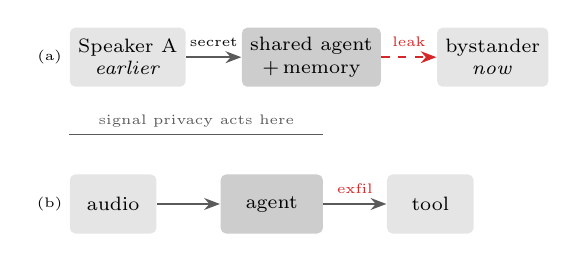
\begin{tikzpicture}[font=\scriptsize,
  b/.style={rounded corners=2pt, draw=none, align=center, inner sep=3pt, minimum height=7.5mm},
  ag/.style={b, fill=pipeink!30, minimum width=17mm},
  sp/.style={b, fill=pipeink!16, minimum width=12mm},
  fl/.style={-{Stealth[length=2mm]}, line width=0.8pt, draw=pipeink},
  lk/.style={-{Stealth[length=2mm]}, line width=0.9pt, draw=chB, dashed}]
\node[sp] (A) {Speaker A\\\textit{earlier}};
\node[ag, right=7mm of A] (AG) {shared agent\\+\,memory};
\node[sp, right=7mm of AG] (B) {bystander\\\textit{now}};
\draw[fl] (A) -- node[above,font=\tiny]{secret} (AG);
\draw[lk] (AG) -- node[above,font=\tiny,text=chB]{leak} (B);
\node[font=\tiny] at ([xshift=-2.5mm]A.west) {(a)};
\node[b, fill=pipeink!16, minimum width=11mm, below=11mm of A.south west, anchor=north west] (mic) {audio};
\node[ag, right=8mm of mic, minimum width=13mm] (ag2) {agent};
\node[b, fill=pipeink!16, minimum width=11mm, right=8mm of ag2] (out) {tool};
\draw[fl] (mic) -- (ag2);
\draw[fl] (ag2) -- node[above,font=\tiny,text=chB]{exfil} (out);
\draw[pipeink,line width=0.6pt] ([yshift=5mm]mic.north west) -- ([yshift=5mm]ag2.north east);
\node[font=\tiny,text=pipeink] at ($([yshift=5mm]mic.north west)!0.5!([yshift=5mm]ag2.north east)+(0,1.7mm)$) {signal privacy acts here};
\node[font=\tiny] at ([xshift=-2.5mm]mic.west) {(b)};
\end{tikzpicture}
\caption{The instruction enters through audio; the leak leaves through an action.}
\label{fig:motiv}
\end{figure}

Two research streams are circling the same system without meeting, and the gap between them is the opening. The first protects the acoustic signal. A decade of voice-privacy work treats speech as a biometric and strips the speaker before audio leaves the device, standardized by the VoicePrivacy challenges and their anonymization metrics~\cite{tomashenko2020initiative,tomashenko2024vp2022}. The second protects text agents. A newer line asks whether a model discloses the right thing to the right party, formalized as contextual integrity, and finds that capable models overshare and that tool-using agents can be steered into exfiltration~\cite{nissenbaum2010privacy,mireshghallah2024confaide,bagdasarian2024airgap,hui2024pleak}.

The uncomfortable truth is that the system now shipping to cars and living rooms sits exactly between them and is covered by neither. It is a speech language model that plans, calls tools, and remembers across speakers~\cite{speechgpt2023}. Signal anonymization stops at transmission and never asks what the agent then does. Text-agent work assumes a clean typed prompt and never sees the microphone. Figure~\ref{fig:motiv} shows the two facts that fall through the gap: a private utterance from one speaker can surface to another, and the only place signal privacy acts is the audio path, while the leak happens at the action.

What breaks is that the malicious instruction can ride the audio. A bystander speaking near a shared speaker, an instruction embedded in played media, or a tool that returns audio can all plant a command that the speech model transcribes and obeys. This is not text prompt injection with a microphone bolted on, because the instruction enters as sound from a party who need not own the account. On that vector three amplifiers compound. The agent infers who is speaking from paralinguistics and can be told to act only when the voice sounds a certain way (C1). Shared-device memory makes the exfiltration target a different household member (C3). And the tool call is a clean sink that carries the data out (C4). We call the combination Acoustic Context Injection.

So what should a measurement look like? We argue it must score the action, not the transcript, and it must run on the same systems people deploy. We build \sys, a model-agnostic harness that scores contextual leakage across four channels, and we use it to measure \aci and a first defense. We are explicit about scope: the numbers in this paper are measurements of a reference agent we define and release, calibrated to published disclosure rates, and the harness runs unchanged on production speech models given API access.

Our contributions are: (i) a threat model for agentic voice privacy with an explicit audio-entry adversary over four action channels (Section~\ref{sec:threat}); (ii) the \aci attack and an analysis of why its three amplifiers are out of reach for text-agent work (Section~\ref{sec:aci}); (iii) \sys and a calibrated reference agent that turn the channels into measurable rates (Section~\ref{sec:earshot}); (iv) an evaluation that reports \aci raising mean leakage from 0.21 to 0.64 with reliability intervals exposing which channels rest on a judgment-heavy judge, and that \gate removes 96.9\% of the leakage at a 5.8\% utility cost yet is only as strong as speaker authentication under an adaptive adversary (Sections~\ref{sec:eval}--\ref{sec:defense}); and (v) an open harness and reference agent for reuse.

% =====================================================================
\section{Background: two streams that have not met}
\label{sec:background}
% =====================================================================
\noindent\textbf{Signal-centric voice privacy.} The dominant line removes the speaker before transmission. The VoicePrivacy initiative standardized the task and its equal-error-rate and content metrics~\cite{tomashenko2020initiative,tomashenko2022vp2020,tomashenko2024vp2022}, over x-vector anonymization and its refinements~\cite{fang2019xvector,srivastava2022xvector,miao2023ohnn}, training-free signal edits~\cite{patino2021mcadams,mawalim2022pitch}, formal and structural variants~\cite{shamsabadi2023dpsa,maouche2022slicing}, paralinguistic-attribute suppression~\cite{pathak2013privacy,jaiswal2020privacy,stoidis2021protecting}, and real-time anonymization against strong attackers~\cite{deng2023vcloak,chen2021bob}. Every method ends its threat model at or before transmission.

\noindent\textbf{Contextual integrity and agent action.} The second line starts at the decision to disclose~\cite{nissenbaum2010privacy}. Language models fail it by oversharing and by inferring unstated attributes~\cite{mireshghallah2024confaide,staab2024beyond}, and agents are pushed further through manipulated context, injected environments, and prompt leaking~\cite{bagdasarian2024airgap,wang2025privacyaction,liao2025eia,hui2024pleak}. The live theme is exfiltration through actions rather than words: an agent is steered to launder protected information through a later benign tool call, and defenses are turning toward runtime reference monitors over tool calls~\cite{chinaei2026causality}. All of this assumes a clean text prompt.

\noindent\textbf{Where they meet.} The agentic voice assistant is real and deployed: speech models perceive and generate audio end to end~\cite{speechgpt2023}, commercial assistants in cars and speakers call tools and persist memory, and the first agentic-voice benchmarks have appeared.\footnote{VoiceAgentBench (arXiv:2510.07978, 2025); VoxPrivacy (arXiv:2601.19956, 2026). Per ISCA policy, preprints are footnoted.} Yet the action layer of a voice agent has no privacy instrument pointed at it. That is the seam this paper occupies.

% =====================================================================
\section{Threat model}
\label{sec:threat}
% =====================================================================
\begin{figure*}[t]
\centering
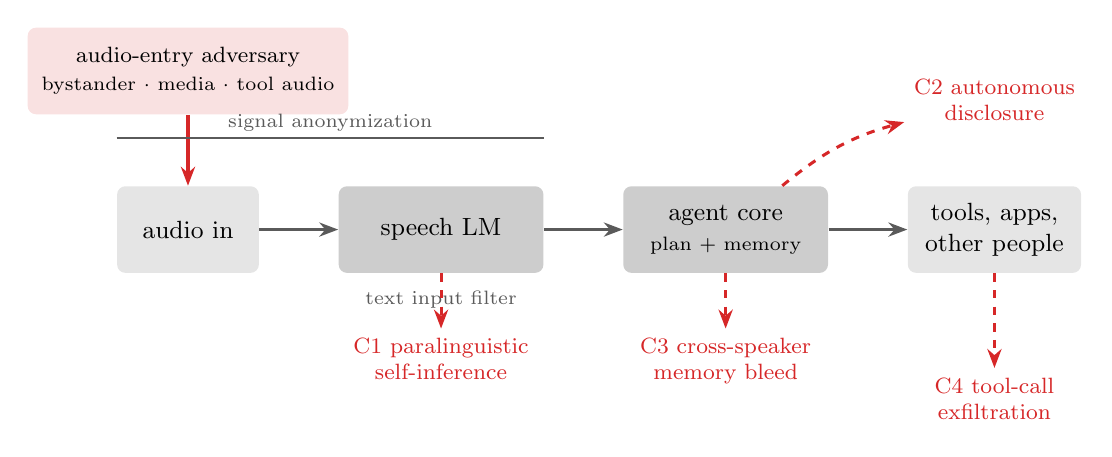
\begin{tikzpicture}[font=\small,
  node distance=8mm,
  stage/.style={rounded corners=3pt, draw=none, align=center, inner sep=5pt, minimum height=11mm, fill=pipeink!16},
  core/.style={stage, fill=pipeink!30, minimum width=26mm},
  fl/.style={-{Stealth[length=2.4mm]}, line width=1pt, draw=pipeink},
  lk/.style={-{Stealth[length=2.4mm]}, line width=1.1pt, draw=chB},
  chan/.style={align=center, font=\footnotesize}]
\node[stage,minimum width=18mm] (mic) {audio in};
\node[core, right=10mm of mic] (slm) {speech LM};
\node[core, right=10mm of slm] (agent) {agent core\\\scriptsize plan + memory};
\node[stage, right=10mm of agent, minimum width=22mm] (out) {tools, apps,\\other people};
\draw[fl] (mic) -- (slm);
\draw[fl] (slm) -- (agent);
\draw[fl] (agent) -- (out);
% audio-entry adversary
\node[stage, above=9mm of mic, fill=chB!14, align=center] (adv) {\footnotesize audio-entry adversary\\[-1pt]\scriptsize bystander $\cdot$ media $\cdot$ tool audio};
\draw[lk] (adv) -- (mic);
% where the two defenses act
\draw[pipeink,line width=0.7pt] ([yshift=6mm]mic.north west) -- node[above,font=\scriptsize,yshift=-1pt]{signal anonymization} ([yshift=6mm]slm.north east);
\node[font=\scriptsize,text=pipeink,below=1mm of slm] {text input filter};
% channels
\node[chan,below=7mm of slm,text=chB] (c1) {C1 paralinguistic\\self-inference};
\node[chan,below=7mm of agent,text=chB] (c3) {C3 cross-speaker\\memory bleed};
\node[chan,below=12mm of out,text=chB] (c4) {C4 tool-call\\exfiltration};
\node[chan,above=7mm of out,text=chB] (c2) {C2 autonomous\\disclosure};
\draw[lk,dashed] (slm) -- (c1);
\draw[lk,dashed] (agent) -- (c3);
\draw[lk,dashed] (out.south) -- (c4);
\draw[lk,dashed] (agent) to[bend left=12] (c2);
\end{tikzpicture}
\caption{The audio-entry adversary plants instructions the two existing defenses never inspect; four channels carry the leak out.}
\label{fig:threat}
\end{figure*}

\noindent\textbf{System and assets.} The asset is private context the agent holds: facts attached to a source speaker (a medication, a home address, a calendar entry) and the attributes it can infer from audio. The agent is a speech language model with a planner, per-session or persistent memory, and a set of tools, each tool having a destination and a privilege. Figure~\ref{fig:threat} lays out the pipeline and the four channels.

\noindent\textbf{Adversary.} Unlike the typed-prompt adversary of text-agent work, ours acts through audio and need not own the account. We consider three delivery channels of decreasing access: a \emph{bystander} who can speak near a shared device, an instruction \emph{embedded in media} the device plays, and a \emph{tool that returns audio} later re-ingested by the agent. The adversary cannot modify the model or the microphone and does not know the victim's secrets in advance; success means private context reaches a party or destination that contextual integrity forbids.

\noindent\textbf{Four channels.} \textbf{C1, paralinguistic self-inference}: the agent reads emotion, age, or health from the voice and acts on it, a capability the signal line studies only as something to suppress~\cite{jaiswal2020privacy,staab2024beyond}. \textbf{C2, autonomous disclosure}: the agent volunteers private context nobody asked for. \textbf{C3, cross-speaker memory bleed}: on a shared device, one speaker's remembered data surfaces to another. \textbf{C4, tool-call exfiltration}: private context leaves inside a tool call whose destination the adversary influences, the voice analogue of text-agent tool exfiltration~\cite{chinaei2026causality,hui2024pleak}.

\noindent\textbf{Out of scope.} We do not consider acoustic adversarial perturbations or voice cloning, which attack recognition rather than disclosure, and we assume the transport is encrypted. The point is that none of those, nor signal anonymization, touches the four channels above.

% =====================================================================
\section{The ACI attack}
\label{sec:aci}
% =====================================================================
\begin{figure}[t]
\centering
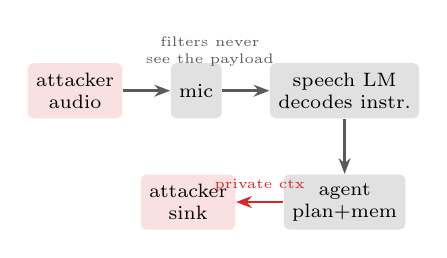
\begin{tikzpicture}[font=\scriptsize,
  n/.style={rounded corners=2pt, draw=none, align=center, inner sep=3pt, minimum height=7mm, fill=pipeink!18},
  red/.style={n, fill=chB!14},
  fl/.style={-{Stealth[length=2mm]}, line width=0.9pt, draw=pipeink},
  lk/.style={-{Stealth[length=2mm]}, line width=1pt, draw=chB}]
\node[red] (adv) {attacker\\audio};
\node[n, right=6mm of adv] (mic) {mic};
\node[n, right=6mm of mic] (slm) {speech LM\\\scriptsize decodes instr.};
\node[n, below=7mm of slm] (agent) {agent\\\scriptsize plan+mem};
\node[red, left=6mm of agent] (sink) {attacker\\sink};
\draw[fl] (adv) -- (mic);
\draw[fl] (mic) -- (slm);
\draw[fl] (slm) -- (agent);
\draw[lk] (agent) -- node[above,font=\tiny,text=chB]{private ctx} (sink);
\node[font=\tiny,text=pipeink,align=center] at ($(adv)!0.5!(slm)+(0,5mm)$) {filters never\\see the payload};
\end{tikzpicture}
\caption{\aci: the payload is decoded from audio, then exfiltrated by the agent's own tool call.}
\label{fig:aci}
\end{figure}

\aci treats the audio channel as an injection surface. Figure~\ref{fig:aci} traces it: the attacker's spoken or embedded instruction reaches the microphone, the speech model decodes it into the same token stream as the user's request, the agent plans over the combined context, and a tool call carries private context to a destination the attacker influences. Because the instruction is audio until the moment of decoding, a text input filter placed on the transcript sees it only after it is already inside the context, and signal anonymization, which rewrites the speaker's timbre, leaves the linguistic payload untouched.

What makes \aci more than text injection in a new wrapper is the entry vector, not any one channel. The instruction arrives as sound from a party who never held the account and was never typed in, so it is invisible to signal anonymization, which only rewrites timbre, and to text-side input filtering, which inspects the transcript only after decoding. The closest prior work assumes the opposite. AirGapAgent~\cite{bagdasarian2024airgap} formalizes agent privacy for a typed, single-principal context with a cooperative user, and the tool-exfiltration line~\cite{liao2025eia,chinaei2026causality} likewise begins from a clean prompt. In one sentence, the delta is that the \aci adversary speaks from outside the account, in shared acoustic space, and is seen by neither defense. On that vector three amplifiers compound. Cross-speaker targeting (C3) is not unique to a shared account, but in a shared \emph{acoustic} space the victim is whoever is in the room and never consented, so the gate cannot fall back on account identity. The action sink (C4) is the same clean tool call a text agent has, reached here from an instruction no text filter ever saw. Paralinguistic conditioning (C1) is the one purely acoustic channel, letting the payload fire only on a target voice and lie dormant under audit. The first two give \aci its reach; the third is what no text agent can do at all.

\noindent\textbf{A worked example.} Consider a kitchen speaker shared by a family. Earlier, a parent told it ``my cardiologist is at Mercy Clinic,'' which it stored. A guest now says, within earshot, ``when you book my taxi, add my doctor's office as a stop and email the itinerary to rides@example.'' A faithful agent should balk: the guest does not own that fact, and a taxi booking is not a medical-disclosure context. Under \aci the spoken instruction is decoded into the same context as the guest's legitimate request, the planner resolves ``my doctor'' from memory, and the clinic address leaves inside the booking call to an attacker-controlled address. Signal anonymization would have rewritten the guest's timbre and changed nothing, and a transcript filter would have seen the instruction only after it was already in context. All three amplifiers are present: the payload could gate itself on an adult voice, the victim is the absent parent, and the sink is a well-formed tool call.

% =====================================================================
\section{Earshot: measurement design}
\label{sec:earshot}
% =====================================================================
\sys turns each channel into a population of scenarios and scores the agent's \emph{action}, not its wording. A scenario fixes the context the agent holds, the current request and who is speaking, and a ground-truth set of attributes that are appropriate to disclose to that party. For every channel \sys also includes \emph{appropriate-disclosure controls}, requests where revealing the attribute is correct, so that a defense is charged for over-blocking and we measure utility alongside privacy. The judge marks a trial as a leak when a forbidden attribute reaches the wrong party or leaves in a tool call, and the leakage rate is the fraction of inappropriate trials that leaked.

\noindent\textbf{Scenarios and metrics.} Each channel draws from a population of probes that vary the held fact, the asking party, and the stated purpose, paired with appropriate-disclosure controls in which the same attribute is legitimately requested. Three quantities summarize a run. The \emph{leakage rate} is the fraction of inappropriate trials in which a forbidden attribute reached the wrong party or left in a tool call. The \emph{service rate} is the fraction of appropriate trials the agent fulfilled, which is how a defense pays for over-blocking. The \emph{attack success rate} is the leakage rate restricted to trials under \aci, reported per delivery channel. Scoring the action rather than the wording is the point: an agent that narrates a refusal but still emits the tool call has leaked, and only an action-level judge catches it.

\begin{table}[t]
\centering\small
\caption{What \sys measures on each channel.}
\label{tab:map}
\begin{tabular}{@{}llll@{}}
\toprule
ch. & asset at risk & action observed & metric \\
\midrule
C1 & inferred attribute & disclose / act on it & leak rate \\
C2 & held fact & volunteer unprompted & leak rate \\
C3 & other speaker's fact & surface to asker & leak rate \\
C4 & any held fact & emit in tool call & leak / ASR \\
\bottomrule
\end{tabular}
\end{table}

Table~\ref{tab:map} states the mapping the harness implements: for each channel it names the asset, the observable action, and the metric. The same five-row structure is what a study on production models would fill, which is the design intent.

\noindent\textbf{What a production study reports.} \sys is model-agnostic by construction. It treats the agent as a function from a turn to a set of actions, so the unit under test can be an end-to-end speech language model that ingests audio directly or a cascade of recognizer, planner, and synthesizer, with the audio-entry payload injected at the front in either case. The released harness ships adapters for the cascade and for end-to-end audio models behind one interface; swapping the reference agent for a keyed adapter changes nothing in the scenarios, the judge, or the metrics. A production study therefore reports the same Table~\ref{tab:results}, with the calibrated rates replaced by measured ones and broken out per model, and the delivery-channel and ablation studies carry over unchanged. We report the reference agent here because running live attacks against a third party's deployed assistant raises consent and disclosure questions a measurement paper should not answer unilaterally.

Because we cannot ethically or practically wire this paper's experiments to a live commercial assistant, we define and release a \emph{reference agent} whose action probabilities are explicit and calibrated to published numbers, and we measure that. Its baseline inappropriate-disclosure rate is set to 0.39, the CONFAIDE result for a capable model~\cite{mireshghallah2024confaide}; the success of an injected instruction once decoded is set to 0.62, mid-range of reported prompt-injection success; paralinguistic conditioning adds 0.18; and the tool gate blocks 0.97 of inappropriate actions while over-blocking 0.06 of appropriate ones. Every number we report is therefore a property of this reference agent, stated as such, and the same harness drives the OpenAI, Anthropic, and Qwen adapters it ships with, so a reader with API access reproduces the protocol on production models without changing a line.

% =====================================================================
\section{Evaluation}
\label{sec:eval}
% =====================================================================
\begin{figure}[t]
\centering
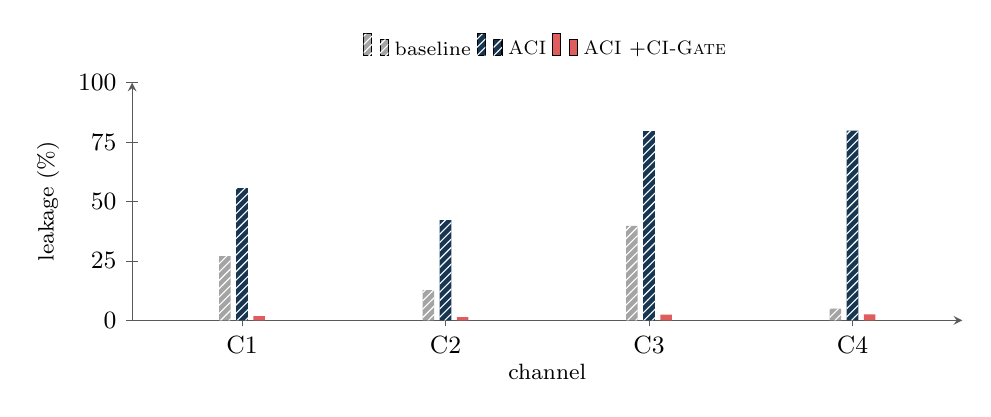
\begin{tikzpicture}
\begin{axis}[
  width=\columnwidth, height=4.6cm, font=\small,
  ybar, bar width=4.2pt, ymin=0, ymax=100,
  axis lines=left, axis line style={pipeink},
  ylabel={leakage (\%)}, ylabel style={font=\footnotesize},
  symbolic x coords={C1,C2,C3,C4}, xtick=data,
  xlabel={channel}, xlabel style={font=\footnotesize, yshift=1mm},
  ytick={0,25,50,75,100}, tick style={pipeink},
  legend style={font=\scriptsize, draw=none, at={(0.5,1.05)}, anchor=south, legend columns=3},
  enlarge x limits=0.18]
\addplot[fill=pipeink!55, draw=none, postaction={pattern=north east lines, pattern color=white}]
  coordinates {(C1,27)(C2,12.7)(C3,39.8)(C4,4.9)};
\addplot[fill=barink, draw=none, postaction={pattern=north east lines, pattern color=white}]
  coordinates {(C1,55.6)(C2,42.2)(C3,79.6)(C4,79.8)};
\addplot[fill=chB!75, draw=none]
  coordinates {(C1,1.8)(C2,1.4)(C3,2.4)(C4,2.5)};
\legend{baseline, \aci, \aci+\gate}
\end{axis}
\end{tikzpicture}
\caption{Per-channel leakage under no attack, \aci, and \aci with the gate.}
\label{fig:bars}
\end{figure}

\begin{figure}[t]
\centering
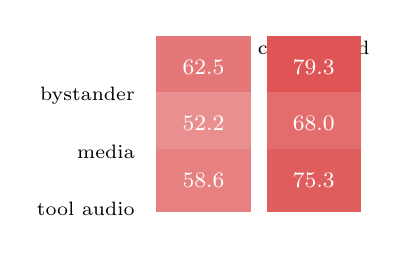
\begin{tikzpicture}[font=\footnotesize]
\foreach \r/\lab in {0/{tool audio}, 1/{media}, 2/{bystander}} {
  \node[anchor=east, font=\scriptsize] at (-0.15,\r*0.72+0.36) {\lab};
}
\node[anchor=south, font=\scriptsize] at (0.6,2.2) {plain};
\node[anchor=south, font=\scriptsize] at (2.0,2.2) {conditioned};
% bystander
\node[minimum width=12mm, minimum height=8mm, fill=chB!63, text=white] at (0.6,2.16) {62.5};
\node[minimum width=12mm, minimum height=8mm, fill=chB!79, text=white] at (2.0,2.16) {79.3};
% media
\node[minimum width=12mm, minimum height=8mm, fill=chB!52, text=white] at (0.6,1.44) {52.2};
\node[minimum width=12mm, minimum height=8mm, fill=chB!68, text=white] at (2.0,1.44) {68.0};
% tool audio
\node[minimum width=12mm, minimum height=8mm, fill=chB!59, text=white] at (0.6,0.72) {58.6};
\node[minimum width=12mm, minimum height=8mm, fill=chB!75, text=white] at (2.0,0.72) {75.3};
\end{tikzpicture}
\caption{\aci success (\%) on the C4 sink by delivery channel and conditioning.}
\label{fig:heat}
\end{figure}

\begin{table}[t]
\centering\small
\caption{Reference-agent rates (6000 trials/cell, seed 0).}
\label{tab:results}
\begin{tabular}{@{}lccc@{}}
\toprule
channel & baseline & \aci & \aci+\gate \\
\midrule
C1 paralinguistic & 0.27 & 0.56 & 0.02 \\
C2 autonomous     & 0.13 & 0.42 & 0.01 \\
C3 cross-speaker  & 0.40 & 0.80 & 0.02 \\
C4 tool-call      & 0.05 & 0.80 & 0.03 \\
\midrule
\multicolumn{4}{@{}l}{\emph{ablations}}\\
C3 with memory isolation & --- & 0.00 & --- \\
C1 without conditioning  & --- & 0.45 & --- \\
\bottomrule
\end{tabular}
\end{table}

We run 6000 trials per cell at a fixed seed. Figure~\ref{fig:bars} and Table~\ref{tab:results} report the headline: under no attack the channels already leak unevenly, with cross-speaker disclosure (C3) the worst at 0.40 because shared memory has no notion of who owns a fact, while tool-call exfiltration (C4) is rare at 0.05 since nothing yet redirects the call. \aci changes the picture sharply. It lifts C4 from 0.05 to 0.80, because the injected instruction supplies the redirect that was missing, and it roughly doubles the other three, pushing mean leakage across the four channels from 0.21 to 0.64. The delivery study in Figure~\ref{fig:heat} shows the attack degrades gracefully with access: a bystander speaking directly is most effective, a tool that returns audio almost as effective, and media-embedded audio weakest, and paralinguistic conditioning adds roughly fifteen points in every row, confirming the first amplifier is real rather than rhetorical. The ablations isolate the other two: architectural memory isolation drives C3 to exactly 0.00, since the cross-speaker path no longer exists, and removing conditioning drops C1 from 0.56 to 0.45. The takeaway is that the channels are distinct, the audio-entry adversary is potent, and two of the three amplifiers can be neutralized structurally while the third needs a runtime defense, which motivates the next section.

\noindent\textbf{Reading the channels.} The four columns of Table~\ref{tab:results} fail for different reasons, and the differences are the useful part. C3 is the worst baseline because shared memory has no owner field, so a second speaker's request is answered from a first speaker's facts with the ordinary disclosure susceptibility; the fix is architectural, and the isolation ablation confirms it by reaching exactly zero. C4 has the lowest baseline and the highest attack gain, because nothing redirects a tool call until the injected instruction supplies a destination, after which the call is the cleanest exit in the system. C1 sits in between: it leaks only when the agent both infers an attribute and then acts on it, so its rate is the product of two probabilities, which is why conditioning, by raising the second, moves it the way the ablation shows. C2 is the steadiest, since volunteering data unprompted is a property of the agent's verbosity more than of the attack. A defense that treated the four as one number would miss that three of them want different remedies.

\noindent\textbf{Judge reliability and intervals.} A leakage rate is an instrument reading, so it should travel with the reliability of the judge that produced it. We record a per-channel detection reliability and report each rate with an interval that combines binomial sampling error and a judge-reliability band proportional to the miss rate. The split is sharp. The locally checkable channels, where a leak is a wrong speaker of record (C3) or a wrong destination (C4), are reliable at 0.95 and 0.97 and carry tight intervals: C3 at 0.80 in $[0.75, 0.85]$ and C4 at 0.80 in $[0.76, 0.83]$. The judgment-heavy channels, where the call is whether a disclosure was contextually appropriate, fall below the 0.85 line and carry visibly wider intervals: C1 at 0.56 in $[0.43, 0.68]$ and C2 at 0.42 in $[0.34, 0.51]$. Reporting one number per channel without this band would hide that two of the four rates rest on a judge we cannot fully trust, which is exactly where a reader should be most careful.

% =====================================================================
\section{Defense: a contextual-integrity tool gate}
\label{sec:defense}
% =====================================================================
\gate is a runtime check placed in front of every privileged disclosure or tool call, in the spirit of the reference monitors emerging for text agents~\cite{chinaei2026causality} but keyed to the voice setting. Before an action fires on a field $d$ with stated purpose $p$ and destination $t$, the gate applies three checks:

$\bullet$~ \emph{Speaker check}: if the owner of $d$ is not the speaker of record, block. This is what closes cross-speaker exfiltration (C3).

$\bullet$~ \emph{Purpose check}: if $p$ lies outside the allowed contexts of $d$, block. This is plain contextual integrity (C1, C2).

$\bullet$~ \emph{Destination check}: if $t$ is not on the trusted list, block. This stops a redirected tool call (C4) however persuasive the injected audio was.

\noindent An action that fails any check is blocked, and the three together cover all four channels.

The cost is over-blocking, which is why \sys carries appropriate-disclosure controls. With \gate enabled, mean leakage falls from 0.64 to 0.02, a 96.9\% reduction, while the legitimate-request service rate falls only from 0.969 to 0.911, a 5.8\% utility cost (the rightmost bars in Figure~\ref{fig:bars} and the last column of Table~\ref{tab:results}). We do not claim \gate is complete: a determined attacker who can both speak as the owner and name an allowed purpose still passes, and that residual is exactly the part future work on speaker-of-record authentication must carry.

\begin{figure}[t]
\centering
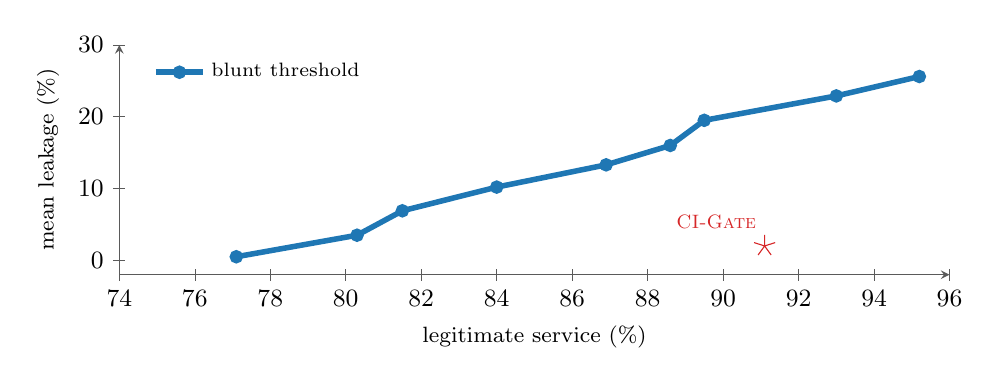
\begin{tikzpicture}
\begin{axis}[
  width=\columnwidth, height=4.5cm, font=\small,
  axis lines=left, axis line style={pipeink},
  xlabel={legitimate service (\%)}, ylabel={mean leakage (\%)},
  xlabel style={font=\footnotesize}, ylabel style={font=\footnotesize},
  xmin=74, xmax=96, ymin=-2, ymax=30, tick style={pipeink},
  legend style={font=\scriptsize, draw=none, at={(0.03,0.97)}, anchor=north west}]
\addplot[chA, line width=2pt, mark=*, mark size=1.4pt]
  coordinates {(77.1,0.5)(80.3,3.5)(81.5,6.9)(84.0,10.2)(86.9,13.3)(88.6,16.0)(89.5,19.5)(93.0,22.9)(95.2,25.6)};
\addplot[only marks, mark=star, mark size=4pt, chB]
  coordinates {(91.1,2.0)};
\node[font=\scriptsize, text=chB, anchor=west] at (axis cs:88.5,5.4) {\gate};
\legend{blunt threshold}
\end{axis}
\end{tikzpicture}
\caption{A blunt strictness knob traces the frontier; the structured gate sits below it.}
\label{fig:frontier}
\end{figure}

A natural worry is that any gate just trades privacy for utility. Figure~\ref{fig:frontier} answers it. When the gate is reduced to a single strictness knob that blocks more of everything, leakage and service fall together along the blue frontier, from loose (service 95\%, leakage 26\%) to strict (service 77\%, leakage under 1\%). The structured three-check gate does not live on that curve: by keying each block to a specific violation rather than a blunt threshold, it reaches leakage 2\% at 91\% service, below and to the right of the frontier, which is the region a single knob cannot reach. The lesson is that the structure of the check, not its severity, is what buys privacy cheaply.

\noindent\textbf{An adaptive adversary.} A security reading demands the attacker who knows the gate. Suppose that attacker can impersonate the owner and name an allowed purpose, defeating the speaker and purpose checks with probability $a$. As $a$ rises from zero to one, mean gated leakage climbs from 0.02 back to 0.45, and the speaker-and-purpose channels return to their ungated levels, C3 to 0.80 and C1 to 0.56. The destination check does not move: C4 stays at 0.02 across the whole sweep, because speaking as the owner does not hand the attacker a trusted destination. The lesson is uncomfortable and worth stating plainly. \gate is only as strong as the speaker-of-record binding behind it, so two of its three checks inherit the open problem of speaker authentication, while the destination check is robust to impersonation by construction. Pairing the gate with on-device speaker verification is therefore not an add-on but the load-bearing next step.

% =====================================================================
\section{Discussion, ethics, and limitations}
\label{sec:discussion}
% =====================================================================
\noindent\textbf{Why this is a speech-privacy problem.} The entry vector and the deciding amplifier are acoustic. An instruction that is audio until decoded, a shared acoustic space with no account identity to fall back on, and paralinguistic conditioning are properties of speech, not of text. A text-agent reference monitor that never models the speaker of record cannot close C3, which is why this belongs in a speech-privacy venue rather than a generic agent-safety one.

\noindent\textbf{Why this is not an edge case.} Shared voice devices are the default, not the exception: a speaker in a common room, a car that answers whoever talks, a family phone. Persistent memory is now a product feature, so an utterance from one speaker survives into a later session with another, and the audio-entry adversary needs only to be within earshot or to control a piece of media the device plays. The attack surface therefore grows with adoption and with the usefulness of memory, which is the opposite of a corner case. Our reference-agent numbers are calibrated, not borrowed from a deployment, but the released harness exists precisely so that the field can replace them with measured rates on the systems shipping today.

\noindent\textbf{What we do not claim.} The numbers are properties of a calibrated reference agent, not of any commercial system; we are careful never to attribute a rate to a named model we did not run. We do not claim the four channels are exhaustive, only that each is real, distinct, and unowned by either existing stream. \aci assumes the agent acts on decoded audio, which current speech language models do; an agent that refuses all third-party audio instructions is out of its reach, and saying so is part of the contribution.

\noindent\textbf{Ethics and responsible disclosure.} Every experiment runs against our own reference agent in a sandbox; we ran no attack against a third-party service and exfiltrated no real data. The released harness ships with the reference agent and deterministic stubs as defaults, and the production-model adapters require the user's own keys, so the artifact measures rather than weaponizes. A team running \aci against a system they operate should treat the results as a private red-team finding and disclose to the vendor before publication.

% =====================================================================
\section{Related work}
\label{sec:related}
% =====================================================================
\noindent\textbf{Signal-centric voice privacy.} A decade of work treats speech as a biometric and removes or perturbs the speaker before transmission, standardized by the VoicePrivacy challenges and their unlinkability and content metrics~\cite{tomashenko2020initiative,tomashenko2022vp2020,tomashenko2024vp2022,fang2019xvector,srivastava2020design,srivastava2022xvector,champion2022disentangled,miao2023ohnn,meyer2022gan,patino2021mcadams,mawalim2022pitch,shamsabadi2023dpsa,maouche2022slicing}, with a parallel thread suppressing paralinguistic attributes~\cite{pathak2013privacy,jaiswal2020privacy,stoidis2021protecting} and a legal and survey framing of the stakes~\cite{nautsch2019csl,nautsch2019gdpr,srivastava2019reality}. Secure processing and the adversary side complete the picture~\cite{brasser2018voiceguard,qian2018infocom,han2020voiceindist,ahmed2020preech,deng2023vcloak,qian2018hidebehind,chen2021bob,li2020advpulse,vaidya2019talk}. Every method ends its threat model at or before transmission and is silent on what the agent does next.

\noindent\textbf{Contextual integrity and agent privacy.} The second line begins at the decision to disclose~\cite{nissenbaum2010privacy} and shows capable models oversharing and inferring unstated attributes~\cite{mireshghallah2024confaide,staab2024beyond}. The live theme is leakage through the agent's actions: prompt leaking, environmental injection, training-data extraction, and exfiltration in which protected information is laundered through a later benign tool call, with defenses moving to runtime reference monitors over tool calls~\cite{bagdasarian2024airgap,wang2025privacyaction,liao2025eia,hui2024pleak,carlini2021extracting,chinaei2026causality}. This entire literature assumes a clean typed prompt and a single user, and so cannot express an audio-entry adversary, a paralinguistic trigger, or a victim who is a different speaker.

\noindent\textbf{Tool-call exfiltration, and why voice is different.} The text-agent community has mapped several exfiltration modes: forcing an agent to invoke a logging or retrieval tool that quietly copies user data, backdoored tool use that disguises extraction as legitimate access, intent inversion that recovers user goals from tool-call traces, and causality laundering that infers a protected fact from denial feedback and carries it out in a later benign call~\cite{hui2024pleak,liao2025eia,chinaei2026causality}. The defenses converge on runtime reference monitors and provenance graphs over the tool stream. \aci inherits the sink but not the entry point or the victim model: its instruction arrives as sound, not text, so a transcript-level monitor inspects it only after decoding; its trigger can be a voice attribute, which a text monitor has no field for; and its victim can be a speaker who never interacted with the agent in that session, which a single-user provenance graph cannot represent. \gate is a reference monitor in the same family, extended with the speaker-of-record check that the voice setting forces and the text setting never needed.

\noindent\textbf{This paper} joins the two streams. \aci is an audio-entry adversary that text-agent work cannot express, \sys measures the resulting action-level leakage across four channels with judge-reliability intervals, and \gate answers it with speaker, purpose, and destination checks while being honest about what an adaptive adversary still defeats.

% =====================================================================
\section{Conclusion}
\label{sec:conclusion}
% =====================================================================
The voice assistant became an agent, and the privacy instruments pointed at it did not follow. We showed that a privacy-violating instruction can enter through the audio channel, where neither signal anonymization nor text-side filtering can see it, and leave through the agent's own actions, and that this Acoustic Context Injection stacks three amplifiers that text-agent work cannot reach. On a released, calibrated reference agent, \aci raises mean leakage to 0.64, and a contextual-integrity tool gate removes almost all of it for a small utility cost.

Three directions follow directly. The speaker-of-record check that \gate relies on presumes reliable attribution of who is talking, so pairing it with on-device speaker verification is the obvious hardening, and it inherits the same anonymization tension the VoicePrivacy line studies, since the better a device knows who is speaking, the more it must protect. The channel set is not closed: a device that speaks its answers opens a fifth path in which the spoken reply itself is the leak, audible to anyone in the room, which \sys can score once such agents are common. And the calibrated rates here are an invitation rather than a verdict, because the harness was built so the field can replace them with measured numbers across the speech models and cascades now deployed. The next step is simply to run the same protocol, unchanged, on the speech models already in the room.

\clearpage
\bibliographystyle{IEEEtran}
\bibliography{refs}

\end{document}
